\section{Variational Quantum Algorithms}
The variational algorithm is one of the most fundamental algorithms 
in quantum computing. It was introduced relatively recently, in 2014. 
The quantum variational algorihtm is one of basic concepts in the field of quantum machine learning. 
When used in \textit{machine learning} tasks, the theoretical algorithm often uses a mix of quantum and classical machines.

The central notion of the Variational Quantum Algorithms - VQA's (I use the plural term, as this is more 
of a family of algorithms instead of one single algorithm) are the parametrized quantum circuits. 

\begin{wrapfigure}{r}{0.3\textwidth}
  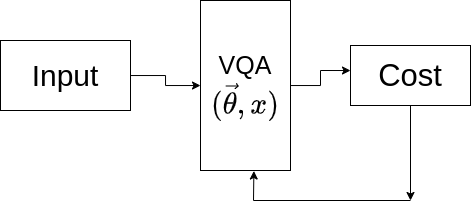
\includegraphics[width=0.3\textwidth]{./basic_vqa.png}
  \caption{}
  \label{fig:basic_vqa}
\end{wrapfigure}

\paragraph{} Parametrized circuits are quantum circuits that contain gates, depending on a certain(s) external parameters. 
For example the $\widehat{R_y}$ gate, as described in \autoref{table:basic_notions}.
These parameters will play the role of these adjustable parameters during machine learning. For example, consider a simple 
linear regression. The parameters of the quantum circuits are analogous to the weights learned during a simple linear 
regression.

The classical VQA follows the basic scheme shown in \autoref{fig:basic_vqa}.

The idea of a VQA is to find a ground state of a Hamiltonian. That is, one recalls one important 
theorems from quantum mechanics - the Variational principle. 
\begin{equation}
  E_0 \leq \frac{\bra{\psi}H\ket{\psi}}{\bra{\psi}\ket{\psi}}
  \label{eq:basic_variational_principle}
\end{equation}
meaning that this inequality is true for any states. Physically speaking, this theorem is quite trivial, 
namely, the ground state has always the smallest energy. The idea of the VQA is therefore to associate a 
Hamiltonian to the problem and to find the state that will minimize the \autoref{eq:basic_variational_principle}.
The cost function will therefore be a funciton of the form 
$\text{Cost}(\theta) = C(\theta) = \bra{\psi}H\ket{\psi}$.
One defines the following theorem (as per \cite{schuld_machine_2018}):
\begin{prettytheorem}[Deterministic quantum model]
  Let $\mathcal{X}$ be the dataset and $U(x,\theta)$ the circuit depending on the data input and the parameters, with $x\in \mathcal{X}$, and $\mathcal{M}$ 
  an observable, e.g. the Hamiltonian. Let $\ket{\psi(x, \theta) \coloneq U(x, \theta)\ket{\psi_0}}$. Then one defines a deterministic 
  quatum model as $f_{\theta} = \bra{\psi(x, \theta)}\mathcal{M}\ket{\psi(x,\theta)}$.
  \label{th:deterministic_quantum_model}
\end{prettytheorem}
This is quite an abstract and general definition. That is, in a general ML algorithm, there exists a target, that one wants to approach. In the case of the 
most general quantum algorithm, it is illustrated by the observable $\mathcal{M}$. The estimation of it is done through the application of the operator $U$ on the input 
state $\ket{\psi}$. One can say that the observable $\mathcal{M}$ is an analogy to the Hamiltonian $H$ discussed before\footnote{Even though the Hamiltonian is \underline{not an observable}.}
Before moving to a concrete example of a Variational algorithm, one defines another (2) theorem(s).
\begin{prettytheorem}[General parametrized circuit]
  A parametrized quantum circuit can be thought of as a unitary operator $U(x,\theta)$. This unitary operator 
  $U(x,\theta)$ can be represented as a sum of a purely parametrized and purely encoding circuits. That is, 
  \begin{equation}
    U(x,\theta) = W_{N+1}\prod_{i=1}^{N}S_i(x_i)W_i(\theta_i)
  \end{equation}
  depicted in circuit \ref{cirq:parametrized_embedded}. In addition, the encoding operator involved in 
  the unitary parametrized 
  operator, encoding a feature $k$ can be written as 
  \begin{equation}
    S_i(x) \equiv S(x_i) \equiv S_i(x_i) = e^{-ix_i\hat{G}_i}
  \end{equation}
  where the operator $G_i \equiv G$ is supposed to be diagonal: $G = \sum_k g_k\ket{g_k}\bra{g_k}$.
  If not, one can always change of basis making use of $P^{\dag}GP$, so that the change of base operators 
  $P^{\dag}$ and $P$ are absorbed into the encoding gates $S_i$.
  \label{th:u_as_s_and_w}
\end{prettytheorem}
\begin{wraptable}[8]{R}{9cm}
  \centering
  \begin{tblr}{c}
    \Qcircuit @C=0.75em @R=1.0em {
      \lstick{\ket{0}} &\qw & \multigate{2}{S_1}  & \qw & \multigate{2}{W_1} &      &\qw&   \multigate{2}{S_{N}} & \multigate{2}{W_{N+1}}   \\
      \vdots           &    & \ghost{S_1}         & \qw & \ghost{W_1}        &\vdots&   &   \ghost{S_{N}}     & \ghost{W_{N+1}}   \\
      \lstick{\ket{0}} &\qw & \ghost{S_1}         & \qw & \ghost{W_1}        &      &\qw&   \ghost{S_{N}}     & \ghost{W_{N+1}}   
  }
\end{tblr}
\caption{}
\label{cirq:parametrized_embedded}
\end{wraptable}

The next theorem is a bit more complex and more mathematical \cite{schuld_machine_2018}. 
This theorem makes a more explicit the expression 
given in \autoref{th:deterministic_quantum_model}. 

\begin{prettytheorem}[Deterministic quantum model (V. 2.0)]
  Let $f_\theta$ be the deterministic quantum model as defined before. Let $U(x,\theta)$ - the parametrized unitary operator 
  as defined above. The features from the $\mathcal{X}$ are also encoded as above. Then, the model is given by 
  \begin{equation}
    f_{\theta}(\vec{x}) = \sum_{\omega_{1}\in \Omega_1} \hdots \sum_{\omega_1 \in \Omega_N} c_{\omega_1 \hdots \omega_N} 
    e^{i\omega_1x_1} \hdots e^{i\omega_Nx_N} 
  \end{equation}
  where the frequency difference $\Omega_i$ is defined to be 
  \begin{equation}
    \Omega_i = \{\lambda_k - \lambda_j \; \big\vert \; k,j\in\{1,...,D\}\}
  \end{equation}
  with $D$ - the dimension of the feature space that the operator $S_i$ maps to.\footnote{
    The sketch of the proof is provided in \cite{schuld_machine_2018}.
  }
  \label{th:deterministic_quantum_model_v2}
\end{prettytheorem}

\paragraph{} In order to get this more straight, one considers the simplest case of the VQA - the variational quantum classifier, 
using the theorems and the concepts we've provied up to now.
We will consider 2 approaches to the variational quantum classifier - first one, considering the usual, plain considerations;
and the second one, using the theorem, that involves the spectrum.

The problem in question is the deterministic quantum model determined with only one encoding circuit $S_{i=1}$ 
and one qubit (one qubit variational quantum classifier).
One takes from \autoref{th:deterministic_quantum_model} $\mathcal{M}$ as $\widehat{\sigma}_z$. Taking the fact that 
$\ket{\psi(x, \theta)} = U(x, \theta)\ket{\psi_0}$, one gets thet the quantum model is given by 
\begin{equation}
  f_\theta(\vec{x}) = \bra{\psi(x,\theta)} \widehat{\sigma_z} \ket{\psi(x,\theta)} = 
  \bra{0}U^{\dag}(x,\theta)\widehat{\sigma_z}U(x,\theta)\ket{0}
\end{equation}

\paragraph{First approach} 
The ansatz of unitary $U(x,\theta)$, is given by 
\begin{equation*}
  U(x, \theta) = \text{Rot}(\theta_1, \theta_2, \theta_3)R_x(x)
\end{equation*}
The deterministic quantum model is, according to definition 
  \begin{align}
  f_\theta(x) = \bra{\psi(x, \theta)}\mathcal{M}\ket{\psi(x, \theta)} = \bra{0}U(x,\theta)^\dag \mathcal{M} U(x,\theta)\ket{0} = \\
  = \bra{0} R_x(x) \text{Rot}(\theta_1, \theta_2, \theta_3)^\dag \widehat{\sigma_z} \text{Rot}(\theta_1, \theta_2, \theta_3)R_x(x) 
  \ket{0} 
  \end{align}
  So one needs to perform a long tideous operation with matrix multiplications involved. The result is given by 
  \begin{equation}
    f_\theta(x) = \cos(\theta_2)\cos(x) - \sin(\theta_1)\sin(\theta_2)\sin(x)
  \end{equation}

Now, one defines the operator $U(x,\theta)$. The choice is more like an arbitrary choice/ansatz. 
Namely, one writes the latter operator in the form given in \ref{th:u_as_s_and_w} 
$U(x, \theta) = W_2(\theta)S_1(x)W_1(\theta)$, where the ansatz-ed operators are defined by 
$W_2(\theta) \coloneq \mathbbm{1}$, $S_1(x) \coloneq R_x(x)$ and 
$W_1(\theta) \coloneq \text{Rot}(\theta_1, \theta_2, \theta_2)$. Since $S_1 \equiv R_x(x)$ and 
$R_x = e^{-i\frac{x}{2}\sigma_x}$, thus, using the representation described in \ref{th:u_as_s_and_w}, 
$G \equiv \nicefrac{\sigma_x}{2}$. One have, however, required $G_i$ to be diagonal. One can, however, 
rewrite the Pauli operator $\sigma_x = V \sigma_z V^\dag$, so that the operator $G_i$ can 
be written in the form of $G_i = V \sigma_z V^\dag$, with $\sigma_z$ being diagonal. 
One can therefore \textit{absorb} these operators $V$, so that the argument in the exponent $e^{-iG}$ 
is diagonal. Using these representations, one can finally write:
\begin{equation}
  \begin{gathered}
    f_\theta(x) = \bra{\psi(\theta, x)}\mathcal{M}\ket{\psi(\theta, x)} \xrightarrow{\mathcal{M} = \sigma_z} \\
    \bra{\psi(\theta, x)}\sigma_z\ket{\psi(\theta, x)} \xrightarrow{\ket{\psi(x,\theta)} = U(\theta, x)\ket{0}}  
    \bra{0} U(x,\theta)^{\dag} \sigma_z U(x, \theta) \ket{0} = \\
    = \bra{0}\widehat{\text{Rot}}^\dag R_x^\dag \sigma_z R_x \widehat{\text{Rot}} \ket{0} = 
    \bra{0}\widehat{\text{Rot}}^\dag (e^{-i\frac{x}{2}\sigma_x})^\dag \sigma_z e^{-i\frac{x}{2}\sigma_x} \widehat{\text{Rot}} \ket{0} =
    \\ 
    =\bra{0}\widehat{\text{Rot}}^\dag (e^{-ixV\sigma_z V^\dag })^\dag \sigma_z e^{-ixV\sigma_z V^\dag } \widehat{\text{Rot}} \ket{0} =\\
    =\bra{0}\widehat{\text{Rot}}^\dag (Ve^{-ix\sigma_z }V^\dag)^\dag \sigma_z Ve^{-ix\sigma_z}V^\dag \widehat{\text{Rot}} \ket{0} =
    \bra{0}\widehat{\text{Rot}}^\dag Ve^{ix\sigma_z }V^\dag \sigma_z Ve^{-ix\sigma_z}V^\dag \widehat{\text{Rot}} \ket{0} =\\
  \end{gathered}
  \label{eq:variational_classifier_single_qubit}
\end{equation}
The operators $V$ and $V^\dag$ can therefore be absorbed into the observable $\mathcal{M}=\sigma_z$.
One can now use the theorem \ref{th:deterministic_quantum_model_v2}. And identify the elements 
mentioned in the theorem to those given in \autoref{eq:variational_classifier_single_qubit}.
From that, one sees that 
\begin{equation*}
  \begin{gathered*}
    N=1  \text{ , } \quad \lambda_i \in \{ -\nicefrac{1}{2}, \nicefrac{1}{2} \} \text{ ,} \quad \Omega_1 \equiv \Omega = \{-1, 0, 1\}
  \end{gathered*}
\end{equation*}

One therefore finds the value of the deterministic model
\begin{equation}
  f_\theta(x) = \sum_{\omega_i \in \Omega} c_{\omega_i} e^{i\omega_ix} = 
  c_0 + 2 \real(c_1)\cos(x) + \imaginary(c_2)\sin(x)
\end{equation}
which bizarrely resembles to the fourier series. In addition to that, one observes the 
same form of the obtained result as in the firs method of evaluating the quantum model.

\subsection*{Implementation of basic 1 qubit classifier}
One can now try to implement the basic 1 qubit variational classifier.
For that, one computes the first need to create a dataset. Namely, 
one will create the following dataset:
\begin{minted}[frame=single, linenos=true]{python}
X = np.array([0.2, 0.89, 0.121, 0.56])
Y = np.array([0, 1, 0, 1])
\end{minted}

The \texttt{X} data is the parameter of the $R_x$. What it means is that the gate $R_x$ will \textit{interpret}
the features. An example of it could be that $x$ is e.g. a footbal's team successful passes' percentage and $y$, 
whether the team has won the game.
One defines the ansatz, to be as described above, namely, $U(x,\theta)=\text{Rot}(\theta)R_x(x)$. 
One uses PennyLane to perform the operations:

\begin{listing}[ht!]
  \begin{minted}[frame=single, linenos=true]{python}
    # Define the quantum device
    dev = qml.device("default.qubit", wires=1)
    # Define the ansatz (U(x, theta))
    def ansatz(x, theta):
        qml.Rot(*theta, wires=0)
        qml.RX(x, wires=0)
    # Define the quantum node
    @qml.qnode(dev)
    def circuit(x, theta):
        ansatz(x, theta)
        return qml.expval(qml.PauliZ(0))
    # Define the cost function for the classifier
    def cost(params, X, Y):
        predictions = np.array([circuit(x, params) for x in X])
        return np.mean((predictions - Y) ** 2)
    params = np.random.uniform(size=(3,))
    # Train the classifier
    opt = qml.GradientDescentOptimizer(stepsize=0.1)
    for i in range(100):
        params = opt.step(lambda p: cost(p, X, Y), params)

  \end{minted}
\end{listing}

Let's consider what does this model do. It starts with initializing the default 1 qubit 
circuit. Then, the ansatz is initialized as discussed below. The \texttt{circuit()} evaluates the 
ansatz with inputs \texttt{x} and \texttt{theta}. The \texttt{cost()} funciton, evaluates the error 
between the obtained value of the cirquit with parameters \texttt{theta} and \texttt{x}, and the 
the target value \texttt{y}.
Then, based on that, the gradient is computed (with respect to $\theta$'s) and $\theta$'s are modified accordingly.
In other words, the $X$ are the features that are tried to be learned and adjusted, together with $\theta$'s. 
The $\theta$'s are thus trying to be adjusted so that the function $f_\theta(x) = y$ are the closest to $y$, which is the 
measured Pauli $\widehat{\sigma}_z$.

\begin{wrapfigure}{r}{0.5\textwidth}
  \centering
  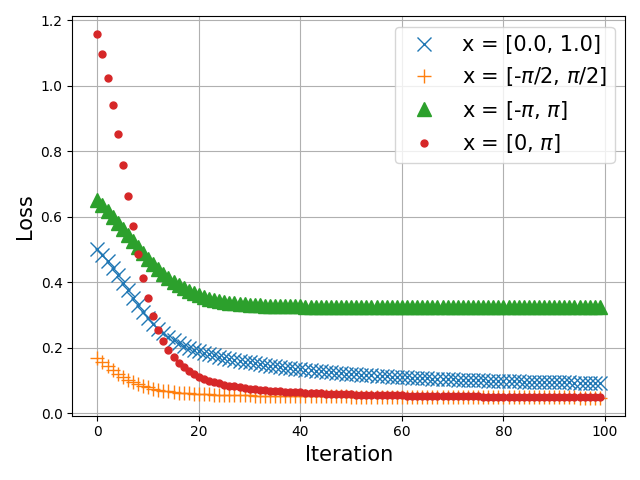
\includegraphics[width=0.5\textwidth]{loss_different_intervals.png}
  \caption{}
  \label{fig:loss_evolution}
\end{wrapfigure}
There are couple of notion that should be mentioned here. First of all, is the input data. 
The data is in form of floats in an interval of $[0,1]$. However, we're working with rotations. So, intuitively, 
there will be some kind of $\sin$, $\cos$ operations involved. Therefore, once again intuitively, the possibly 
desired interval we would want for the input data would be $[0, \pi]$ for $\cos$ 
(since $\cos$ goes over the whole range in this exact interval) and $[-\frac{\pi}{2}, \frac{\pi}{2}]$ for $\sin$ 
(since $\sin$ goes over its whole range in this excat interval).
Thus, we can compare how the loss function evolves with the number of iterations for different possible input intervals. 
This is illustrated in \autoref{fig:loss_evolution}.

Another aspect to discuss is the how is the gradient performed. Namely, in the most general case, the 
updaate mechanism of the parameters $\theta$'s is given by 
\begin{equation}
  \theta_i^{t+1} = \theta_i^{t} - \eta \frac{\partial f_\theta(x)}{\partial \theta_i^{k}}
\end{equation}
One must therefore find a way to estimate the derivative. One way is, of course use the finite differences. 
However, for quantum circuits, there is an another way of finding the derivatives.
















